\chapter{Wstęp}

\section{Używany sprzęt oraz narzędzia}

\begin{itemize}
    \item Stanowisko - \textbf{7}
    \item Oscyloskop - \textbf{MSO3012}
    \item Generator funkcyjny - \textbf{AFG3022B}
    \item Płytka - \textbf{UC-2}
    \item Multimetr - \textbf{5}
\end{itemize}

\section{Jednostki i przedrostki}

\begin{itemize}
    \item 1 Hz (herc) - jednostka miary częstotliwości - 1Hz = $\frac{1}{1s} = 1s^{-1}$
    \item 1 V (wolt) - jednostka potencjału elektrycznego, napięcia elektrycznego i siły elektromotorycznej - 1V = $\frac{1W}{1A}$ ($\frac{wat}{amper}$)
\end{itemize}

\begin{itemize}
    \item k (kilo) = $10^3$
    \item M (mega) = $10^6$
    \item m (mili) = $10^{-3}$
    \item $\mu$ (micro) = $10^{-6}$
    \item n (nano) = $10^{-9}$
\end{itemize}

\section{Charakterystyka układów TTL}
\label{TTL:charakterystyka}

\begin{itemize}
    \item układy pracują w logice dodatniej
    \item logicznemu zeru (L – stan niski) odpowiada napięcie z przedziału:
        \begin{center}
             0 – 0.8 V (sygnały wejściowe) \\
             0 – 0.4 V (sygnały wyjściowe)
        \end{center}
    \item logicznej jedynce (H – stan wysoki) odpowiada napięcie z zakresu:
        \begin{center}
            2.0 – 5 V (sygnały wejściowe) \\
            2.7 – 5 V (sygnały wyjściowe)
        \end{center}
    \item wejście bramki niepodłączone do niczego znajduje się w stanie logicznym 1
    \item układy zasila się napięciem +5 V.
\end{itemize}

\pagebreak
\section{Bramka NAND}
    \begin{itemize}
        \item Symbol:
            \begin{figure}[H]
                \centering
                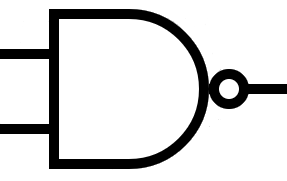
\includegraphics[scale=0.5]{img/schemes/NAND_symbol.png}
                \caption{Symbol bramki NAND}
                \label{fig:symbol_NAND}
            \end{figure}
        \item Wyrażenie algebraiczne:
            \begin{equation}
                \label{eq:NAND}
                Y = \overline{AB}
            \end{equation}
        \item Tabela prawdy:
        \begin{center}
            \label{tabela_prawdy:NAND}
            \begin{tabular}{|c|c|>{\columncolor[gray]{0.8}}c|}
                \hline
                A & B & Y \\
                \hline
                0 & 0 & 1 \\
                \hline
                0 & 1 & 1 \\
                \hline
                1 & 0 & 1 \\
                \hline
                1 & 1 & 0 \\
                \hline
            \end{tabular}
        \end{center}
 \end{itemize}
 
\section{Przerzutnik synchroniczny R-S}

\begin{itemize}
    \begin{figure}[H]
        \centering
        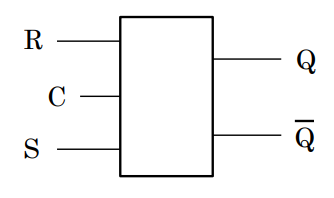
\includegraphics[scale=0.5]{img/schemes/ogolny_schemat_RS.png}
        \caption{Ogólny schemat synchronicznego przerzutnika R-S}
        \label{przerzutnik_RS:ogolny_schemat}
    \end{figure}
    \item Przerzutnik synchroniczny RS ma dodatkowe wejście C do którego doprowadza się sygnał taktujący (zegarowy, synchronizujący). 
    \item Zmiana stanu przerzutnika następuje w chwilach wyznaczonych przez sygnał taktujący. Umożliwia to wstępne przygotowanie sygnałów wejściowych i inicjację zmiany stanu przerzutnika po ustaleniu się tych stanów.
    \item Wyzwalanie zmiany stanu przerzutnika może następować w chwili gdy np. sygnał taktujący zmienia się ze stanu 0 na 1.
    \begin{figure}[H]
        \centering
        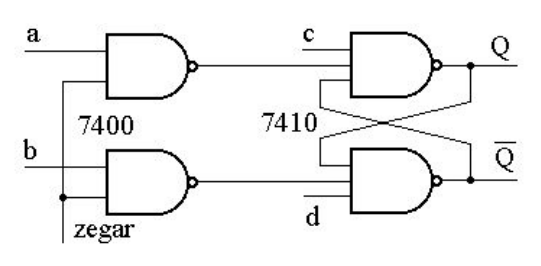
\includegraphics[width=\textwidth]{img/schemes/schemat_RS.png}
        \caption{Schemat przerzutnika R-S używając bramek \textbf{NAND}}
        \label{przerzutnik_RS:schemat}
    \end{figure}
    \item Tabela stanów:
        \begin{center}
            \label{przerzutnik_RS:tabela_stanow}
            \begin{tabular}{|c|c|c|>{\columncolor[gray]{0.8}}c|}
                \hline
                C & S & R & Q \\
                \hline
                1 & 0 & 0 & stan zabroniony\\
                \hline
                1 & 0 & 1 & 1\\
                \hline
                1 & 1 & 0 & 0\\
                \hline
                1 & 1 & 1 & stan pamiętania\\
                \hline
                0 & - & - & stan pamiętania\\
                \hline
            \end{tabular}
        \end{center}
        
    \begin{figure}[H]
        \centering
        \includegraphics{img/schemes/przerzutnik_RS_przykład_przebiegu.png}
        \caption{Przykładowy przebieg czasowy}
        \label{przerzutnik_RS:przebieg}
    \end{figure}
\end{itemize}

\section{Przerzutnik JK}

\begin{itemize}
    \begin{figure}[H]
        \centering
        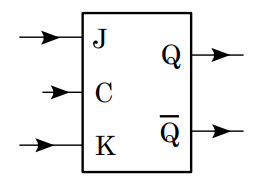
\includegraphics[scale=0.5]{img/schemes/ogolny_schemat_JK.png}
        \caption{Ogólny schemat synchronicznego przerzutnika JK}
        \label{przerzutnik_JK:ogolny_schemat}
    \end{figure}
    \item Wejścia informacyjne J i K odpowiadają wejściom S i R przerzutnika RS.
    \item Przerzutnik JK nie ma stanów wejściowych niedozwolonych. 
    \item W przypadku jednoczesnego podania sygnałów 1 na wejścia J i K, stan przerzutnika zmieni się na przeciwny (w chwili wyzwolenia sygnałem taktującym).
    \item Tabela stanów:
        \begin{center}
            \label{przerzutnik_JK:tabela_stanow}
            \begin{tabular}{|c|c|c|>{\columncolor[gray]{0.8}}c|}
                \hline
                C & J & K & Q \\
                \hline
                0$\uparrow$ & 0 & 0 & stan się nie zmienia\\
                \hline
                0$\uparrow$ & 0 & 1 & 0\\
                \hline
                0$\uparrow$ & 1 & 0 & 1\\
                \hline
                0$\uparrow$ & 1 & 1 & stan zmienia się na przeciwny\\
                \hline
            \end{tabular}
        \end{center}
    \begin{figure}[H]
        \centering
        \includegraphics{img/schemes/przerzutnik_JK_przykład_przebiegu.png}
        \caption{Przykładowy przebieg czasowy}
        \label{przerzutnik_JK:przebieg}
    \end{figure}
\end{itemize}

\section{Przerzutnik D ('latch')}

\begin{itemize}
    \begin{figure}[H]
        \centering
        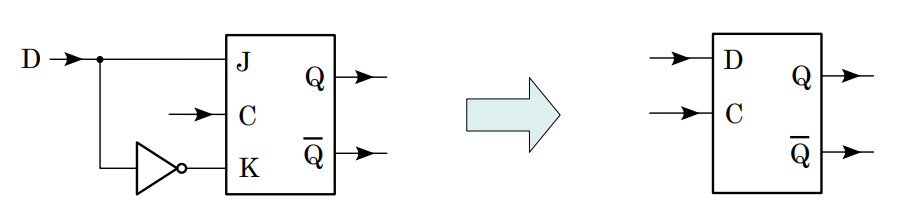
\includegraphics[scale=0.5]{img/schemes/ogolny_schemat_D.png}
        \caption{Ogólny schemat synchronicznego przerzutnika D}
        \label{przerzutnik_D:ogolny_schemat}
    \end{figure}
    \item Przerzutnik D zapamiętuje stan wejścia D w chwili impulsu zegara.
    \item Tabela stanów:
        \begin{center}
            \label{przerzutnik_D:tabela_stanow}
            \begin{tabular}{|c|c|>{\columncolor[gray]{0.8}}c|}
                \hline
                C & D & Q \\
                \hline
                1 & 0 & 0 \\
                \hline
                1 & 1 & 1 \\
                \hline
                0 & - & $Q_{n-1}$ \\
                \hline
            \end{tabular}
        \end{center}
    \begin{figure}[H]
        \centering
        \includegraphics[width=\textwidth]{img/schemes/przerzutnik_D_przykład_przebiegu.png}
        \caption{Przebieg czasowy przerzutnika D \textbf{wyzwalanego poziomem}}
        \label{przerzutnik_D:przebieg_zbocze}
    \end{figure}
    \begin{figure}[H]
        \centering
        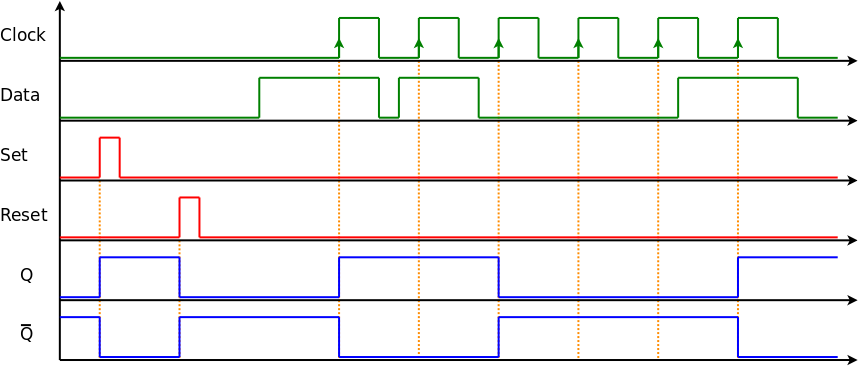
\includegraphics[width=\textwidth]{img/schemes/przerzutnik_D_poziom_przyklad_przebiegu.png}
        \caption{Przebieg czasowy przerzutnika D \textbf{wyzwalanego zboczem}}
        \label{przerzutnik_D:przebieg_poziom}
    \end{figure}
\end{itemize}

\section{Przerzutnik T}

\begin{itemize}
    \begin{figure}[H]
        \centering
        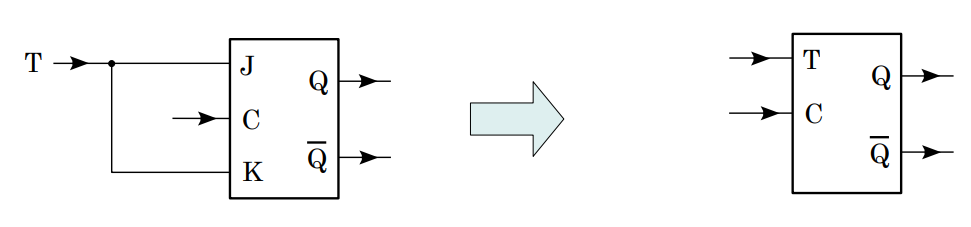
\includegraphics[scale=0.5]{img/schemes/ogolny_schemat_T.png}
        \caption{Ogólny schemat synchronicznego przerzutnika T}
        \label{przerzutnik_T:ogolny_schemat}
    \end{figure}
    \item Przerzutnik T zmienia swój stan na przeciwny w czasie impulsu zegarowego gdy T = 1.
    \item Stan przerzutnika pozostaje bez zmiany gdy T = 0.
    \item W przypadku utrzymywania stanu T = 1, każdy kolejny impuls zegarowy zmienia stan przerzutnika na przeciwny.
    \item Tabela stanów:
        \begin{center}
            \label{przerzutnik_T:tabela_stanow}
            \begin{tabular}{|c|c|>{\columncolor[gray]{0.8}}c|}
                \hline
                C & T & Q \\
                \hline
                0$\uparrow$ & 1 & 0 \\
                \hline
                0$\uparrow$ & 0 & 1 \\
                \hline
                1 & 1 & 0 \\
                \hline
                0 & 0 & stan się nie zmienia \\
                \hline
            \end{tabular}
        \end{center}
    \begin{figure}[H]
        \centering
        \includegraphics[width=\textwidth]{img/schemes/przerzutnik_T_przykład_przebiegu.png}
        \caption{Przykładowy przebieg czasowy}
        \label{przerzutnik_T:przebieg}
    \end{figure}
\end{itemize}

\pagebreak

\section{Licznik}

\begin{itemize}
    \item Licznikem nazywamy układ cyfrowy służący do zliczania impulsów.
    \item Na wyjściu licznika pojawia się zakodowana binarnie liczba impulsów podanych na wejście zliczające. 
    \item Oprócz wejścia impulsów zliczanych, licznik posiada zazwyczaj wejście ustawiające stan początkowy (zerowanie licznika).
    \item Podstawowymi elementami liczników są przerzutniki T. Pojedynczy przerzutnik T pozwala na zliczanie 2 impulsów. 
    \item Najprostszy licznik można zbudować z szeregowo połączonych przerzutników T, z których każdy pod wpływem impulsu zegarowego zmienia swój stan na przeciwny do stanu poprzedniego.
    \begin{figure}[H]
        \centering
        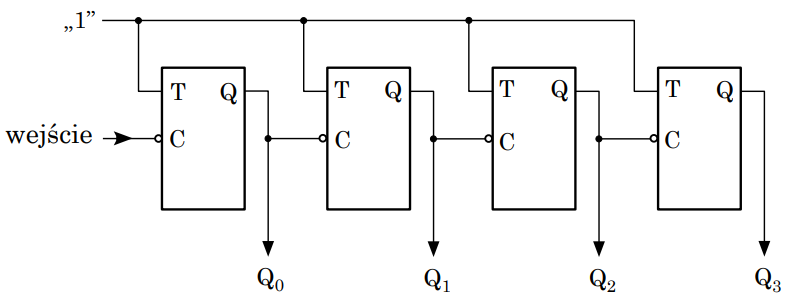
\includegraphics[width=0.8\textwidth]{img/schemes/schemat_licznika_4bitowego.png}
        \caption{Przykładowy licznik 4-bitowy}
        \label{licznik:przykladowy_licznik_4bitowy}
    \end{figure}
    \begin{figure}[H]
        \centering
        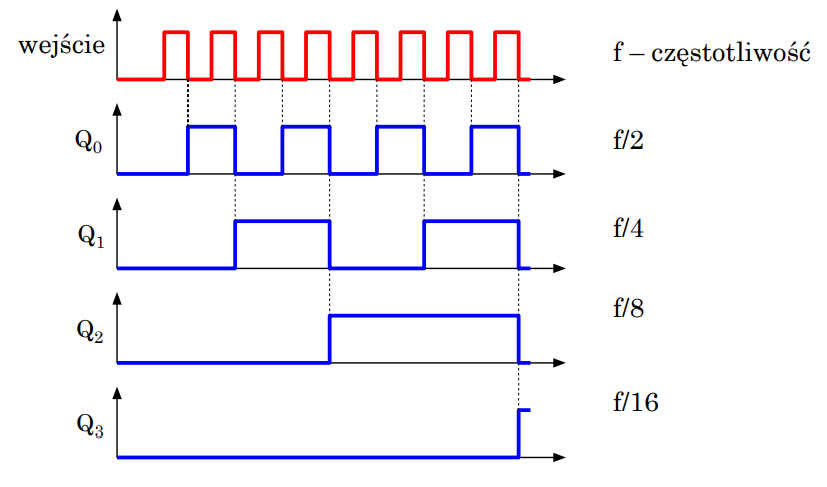
\includegraphics[width=0.8\textwidth]{img/schemes/licznik_przebieg.png}
        \caption{Przebieg czasowy licznika}
        \label{licznik:przebieg}
    \end{figure}
\end{itemize}

\section{Rejestry}

\begin{itemize}
    \item Rejestry służą do przechowywania informacji cyfrowej zapisanej w kodzie binarnym.
    \item Wpisana do rejestru informacja przechowywana jest do chwili wprowadzenia kolejnej, nowej informacji. Informacja ta może być również dostępna do odczytu.
    \item Ze względu na sposób wprowadzania i wyprowadzania informacji rejestry dzielimy na:
        \begin{itemize}
            \item szeregowe – wejście i wyjście szeregowe (rejestry przesuwające)
            \item równoległe – wejście i wyjście równoległe (rejestry buforowe)
            \item szeregowo-równoległe – wejście szeregowe, wyjście równoległe
            \item równoległo-szeregowe – wejście równoległe, wyjście szeregowe.
        \end{itemize}
    \item Wprowadzanie równoległe – wszystkie bity słowa informacji wprowadzamy jednocześnie, w jednym takcie zegara:
        \begin{figure}[H]
            \centering
            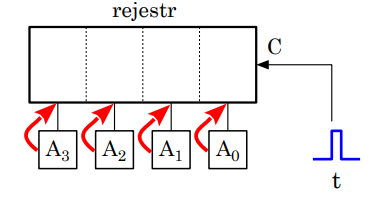
\includegraphics[width=0.6\textwidth]{img/schemes/rejestr_rownolegle.png}
            \label{rejestr:schemat_rownolegle}
        \end{figure}
    \item Wprowadzanie szeregowe – słowo wprowadzamy bit po bicie w kolejnych taktach zegara:
        \begin{figure}[H]
            \centering
            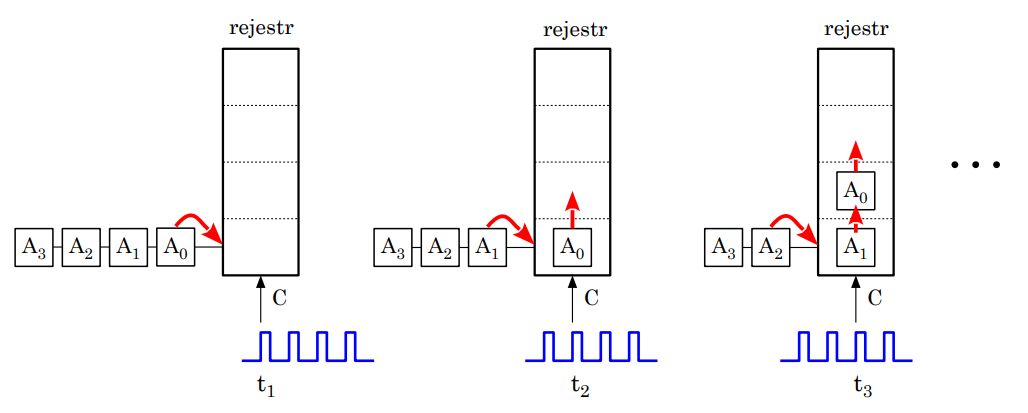
\includegraphics[width=\textwidth]{img/schemes/rejestr_szeregowo.png}
            \label{rejestr:schemat_szeregowo}
        \end{figure}
\end{itemize}